\documentclass[9pt]{beamer}

\usepackage[spanish]{babel}

\usetheme[
  progressbar=frametitle,
  block=fill,
]{metropolis}

% NOTE: Los "frames" que contengan código Python deben tener el
%       la opción "fragile" para que funcionen correctamente.
\usepackage[runall, gobble=auto]{pythontex}

\usepackage{multicol}

\usepackage{booktabs}

\usepackage{mathtools}
\usepackage{units}

\usepackage{tikz}
\usetikzlibrary{babel}

\usepackage{pgfplots}
\pgfplotsset{compat=1.18}

\title{Interpolación segmentaria con \textit{splines}}
\subtitle{}
\author{Francisco González Rubio \and Pedro Pasalodos Guiral%
  \and Mario Vago Marzal}
\date{Curso 2023--2024}
\institute{Universitat de València}

\begin{document}
  % Lista de "imports" (y otros) de PythonTeX.
  \begin{pythontexcustomcode}[begin]{py}
    from splinemaps import *
  \end{pythontexcustomcode}

  {
    % A workaround to hide an overfull \vbox warning produced by
    % the title frame of the Metropolis theme.
    \vfuzz=16pt
    \maketitle
  }

  \begin{frame}{Índice}
    \setbeamertemplate{section in toc}[sections numbered]
    \tableofcontents
  \end{frame}

  \section{Diseñando una línea de metro}
    % \begin{frame}{Diseñando una línea de metro}
  Queremos diseñar una línea de metro alternativa a la línea 4 de
  Metrovalencia. Unir las paradas con \textcolor{orange}{rectas} no es una
  opción ya que el tren no puede girar bruscamente. Debemos conseguir una
  curva \textcolor{red}{suave}.

  \pause

  \begin{multicols}{2}
    \begin{figure}
      \centering
      \includegraphics[width=0.9\linewidth]%
        {figures/metrovalencia4_lerp.png}
      \caption{Línea 4 de Metrovalencia con interpolación lineal.}
    \end{figure}

    \pause

    \begin{figure}
      \centering
      \includegraphics[width=0.9\linewidth]%
        {figures/metrovalencia4.png}
      \caption{Alternativa a la línea 4 de Metrovalencia.}
    \end{figure}
  \end{multicols}
\end{frame}


  \section{Interpolación segmentaria con \textit{splines}}
    % \begin{frame}{Interpolación segmentaria con \textit{splines}}
    Sea $[a, b]$ un intervalo, y sea una partición del intervalo
    \[\Delta = \{a = x_0 < x_1 < \cdots < x_n = b\}.\]
    
    Definiremos el espacio de \textit{splines} como
    \[
        M_2^3(\Delta)
        = {S \in C^2([a, b]) : S|_{[x_{i-1}, x_ i]}
        = q_ i(x) \in \Pi_3, i = 1,\dots, n}.
    \]

    Por lo tanto, el \textit{spline} de una función $f$ es una función
    continua $S$ con primera y segunda derivada continua, tal que
    \[
        S(x_i) = f(x_i), \quad i = 0, \dots, n.
    \]
\end{frame}


  \section{Las condiciones de interpolación}
    % \begin{frame}{Criterios adicionales}
  Para encontrar las $2$ condiciones adicionales, se escoge alguno de los
  siguientes criterios (en función de la información disponible):
  \begin{description}
    \item[\textit{Spline natural}] Si no contamos con información
    adicional, imponemos
    \[
      S''(x_0) = S''(x_n) = 0.
    \]
    \item[\textit{Spline periódico}] Si la función es periódica, imponemos
    \[
      S^{(k)}(x_0) = S^{(k)}(x_n), \quad k = 0, 1, 2. 
    \]
    \item[\textit{Spline} completo] Si conocemos el valor de la segunda
    derivada en los extremos, imponemos
    \[
      S''(x_0) = f''(x_0), \quad S''(x_n) = f''(x_n).
    \]
  \end{description}
\end{frame}


    % Las tres condiciones de interpolación.

    % \input{slides/ejemplo.tex}

  \section{Usando \textit{splines} para parametrizar curvas}
    % \begin{frame}{Usando \textit{splines} para parametrizar curvas}
  Hasta ahora solo sabemos como obtener la curva que interpola
  puntos de \alert{una componente}.

  \pause

  Si tenemos un conjunto de $n$ puntos en $\mathbb{R}^m$ a interpolar,
  procederemos así:
  \begin{enumerate}[<+->]
    \item Determinamos una partición uniforme del intervalo $[0, 1]$ en
    $n - 1$ subintervalos.
    \item Para cada componente, determinamos un \textit{spline} cúbico
    $S_i$ que interpole los puntos de la componente en los nodos de la
    partición.
    \item La curva $S: [0, 1] \longrightarrow \mathbb{R}^m$ definida por
    \[
      S(t) = \left(S_1(t), S_2(t), \ldots, S_m(t)\right)
    \]
    es una curva suave que pasa por los $n$ puntos.
  \end{enumerate}
\end{frame}

    % \begin{frame}{Ejemplo de parametrización con \textit{splines}}
  A continuación se muestra un ejemplo de parametrización con
  \textit{splines} cúbicos. Como se puede observar, la parametrización
  es pasa por todos los puntos de control y es suave en todos los
  trozos.

  \begin{figure}
    \centering
    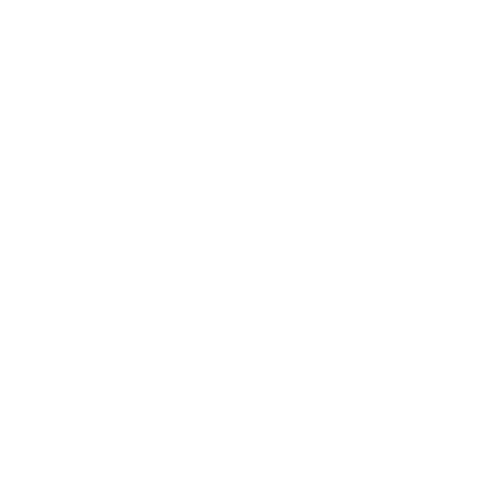
\includegraphics[width=0.45\textwidth]{figures/ejemplo.png}
    \caption{Ejemplo de parametrización con \textit{splines} cúbicos.}
  \end{figure}
\end{frame}


  \section{Comparación con otras técnicas de interpolación}
    % \input{slides/comparacion.tex}

\end{document}
